%!TeX root = main.tex
%!encoding = UTF-8 Unicode

\section{Benchmarking of SiC MOSFET Manufacturers}

Beyond device-parameter studies, the proposed measurement environment also enables benchmarking of semiconductor technologies.
To demonstrate this capability and to establish EM emission as a design dimension in addition to classical trade-offs, a comparative market analysis of four SiC MOSFET devices from different manufacturers is presented.

All evaluated devices are \SI{1200}{V} SiC MOSFETs in D2PAK packages with a current rating of $\SI{60}{A}\pm\SI{5}{A}$ and are operated at $\mi{V}{DC}~=~\SI{800}{V}$ and $\mi{I}{L}~=~\SI{60}{A}$ at room temperature.

\begin{figure}[h]
	\centering
	% \includegraphics[scale = 1]{MeasurementResults/MR_MarketOverview}
	% This file was created by matlab2tikz.
%
%The latest updates can be retrieved from
%  http://www.mathworks.com/matlabcentral/fileexchange/22022-matlab2tikz-matlab2tikz
%where you can also make suggestions and rate matlab2tikz.
%
\definecolor{mycolor1}{rgb}{0.00000,0.44700,0.74100}%
\definecolor{mycolor2}{rgb}{0.85000,0.32500,0.09800}%
\definecolor{mycolor3}{rgb}{0.92900,0.69400,0.12500}%
\definecolor{mycolor4}{rgb}{0.49400,0.18400,0.55600}%
%
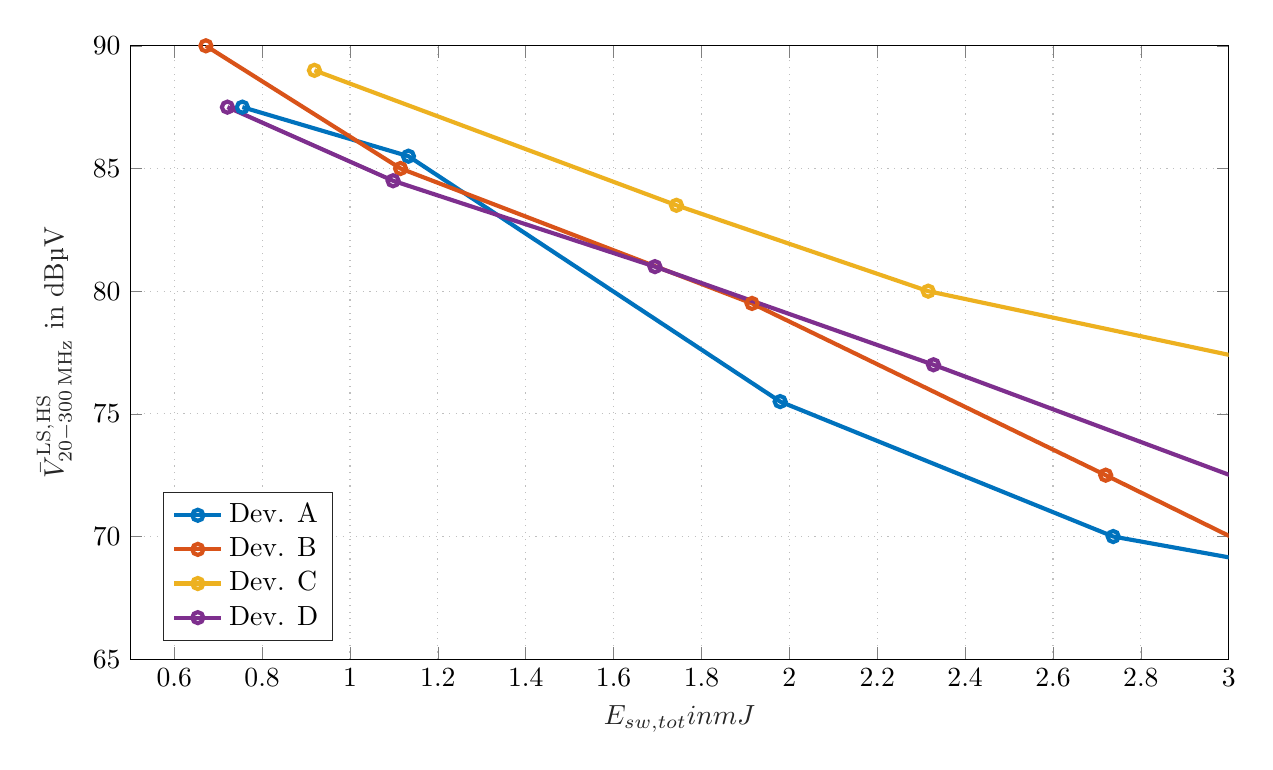
\begin{tikzpicture}

\begin{axis}[%
width=5.492in,
height=3.067in,
at={(0.921in,0.575in)},
scale only axis,
xmin=0.5,
xmax=3,
xlabel style={font=\color{white!15!black}},
xlabel={$\text{E}_{\text{sw,tot}}\text{ in mJ}$},
ymin=65,
ymax=90,
ylabel style={font=\color{white!15!black}},
ylabel={$\bar{V}_\mathrm{20-300\,MHz}^\mathrm{LS,HS}$ in dB\textmu V},
axis background/.style={fill=white},
xmajorgrids,
ymajorgrids,
grid style={dotted},
legend style={at={(0.03,0.03)}, anchor=south west, legend cell align=left, align=left, draw=white!15!black}
]
\addplot [color=mycolor1, line width=1.5pt, mark=o, mark options={solid, mycolor1}]
  table[row sep=crcr]{%
0.755	87.5\\
1.133	85.5\\
1.979	75.5\\
2.737	70\\
3.25	68.34516129\\
};
\addlegendentry{Dev. A}

\addplot [color=mycolor2, line width=1.5pt, mark=o, mark options={solid, mycolor2}]
  table[row sep=crcr]{%
0.672	90\\
1.115	85\\
1.915	79.5\\
2.72	72.5\\
3.25	67.82658393\\
};
\addlegendentry{Dev. B}

\addplot [color=mycolor3, line width=1.5pt, mark=o, mark options={solid, mycolor3}]
  table[row sep=crcr]{%
0.919	89\\
1.743	83.5\\
2.316	80\\
3.25	76.45675266\\
};
\addlegendentry{Dev. C}

\addplot [color=mycolor4, line width=1.5pt, mark=o, mark options={solid, mycolor4}]
  table[row sep=crcr]{%
0.721	87.5\\
1.098	84.5\\
1.694	81\\
2.328	77\\
3.25	70.85333333\\
};
\addlegendentry{Dev. D}

\end{axis}
\end{tikzpicture}%
	\caption{Comparative analysis of EM noise emission performance for SiC MOSFETs from different manufacturers.}\label{fig:MR_CompetitorAnalysis}
\end{figure}

Because a fair comparison at a single operating point is difficult, a gate-resistance sweep of $\mbox{\mi{R}{G,ext} = [1, 5, 10, 20, 30, 50]~\si{\ohm}}$ is performed, with an overvoltage limit of \SI{1200}{V} as the stopping criterion.
% Therefore, a gate-resistance sweep of $\mi{R}{G} = [1, 5, 10, 20, 30, 50]~\si{\ohm}$ is performed, with an overvoltage limit of \SI{1200}{V} as the stopping criterion.
The gate resistance sweep visualizes the trade-off between switching losses and EM noise emission for a given technology.
Hence, for each operating point, the switching loss energy \mi{E}{sw,tot} is calculated together with the average spectral emission of the active and passive switch voltages~\cite{kragl_impact_2024}:

% \begin{equation}
% 	\bar{V}_\mathrm{20-300MHz}^\mathrm{LS,HS} = 20 \log_{10}\left(\frac{\Delta\mi{f}{bin}\sum\limits_{\SI{20}{MHz}}^{\SI{300}{MHz}} \left(\mi{V}{DS,LS}[n] + \mi{V}{DS,HS}[n]\right)}{2\cdot(\SI{300}{MHz} - \SI{20}{MHz})\cdot\SI{1}{\micro V}}\right) 
% \end{equation}

\begin{equation}
	\bar{V}_\mathrm{20-300MHz}^\mathrm{LS,HS} = 20 \log_{10}\frac{\Delta\mi{f}{bin}\sum\limits_{\SI{20}{MHz}}^{\SI{300}{MHz}} \left(\mi{V}{DS,LS}[n] + \mi{V}{DS,HS}[n]\right)}{2\cdot(\SI{300}{MHz} - \SI{20}{MHz})\cdot\SI{1}{\micro V}}
\end{equation}


The resulting comparison, plotted in \fref{fig:MR_CompetitorAnalysis}, shows a clear and expected trend of increasing EM noise emission with decreasing switching energy.
However, the results also show that different devices emit up to \SI{7}{dB} higher average noise levels, with significantly higher differences at specific frequencies.
This establishes EM noise as a design dimension alongside classical trade-offs, and demonstrates the capability of the introduced measurement environment.
